\section{Architecture générale}
\label{archi:general}

\begin{figure}[H]
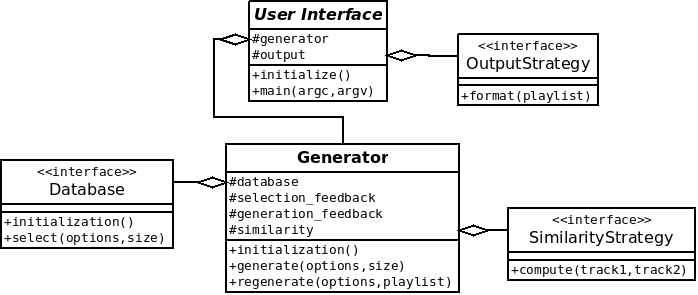
\includegraphics[width=\textwidth]{data/archi/general.png}
\caption{Diagramme général simplifié.}
\end{figure}

L'architecture de \emph{Soundcity} se compose de trois grands modules~:
\begin{itemize}
  \item Le Générateur.
  \item L'Interface Utilisateur.
  \item Le Retour Utilisateur, situé entre les deux.
\end{itemize}

Le module de sortie est un cas un peu particulier car il est principalement
utilisé par l'interface, mais peut être utilisé indépendamment. Il est donc
classé dans le module d'interface, mais sera traité dans une section séparée.

L'avantage de cette modularisation est qu'elle permet d'implémenter plusieurs
interfaces, sans changer la génération, le retour utilisateur, et le format de
sortie.

\section{Communication entre modules~: Morceaux et Options}
\label{archi:communication}

La modularisation discutée dans la section précédente (\ref{archi:general})
demande que les modules puissent communiquer entre eux, pour s'envoyer les
informations nécessaires à leur bon fonctionnement.

\subsection{Morceaux}
\label{archi:communication:track}

Le première structure nécessaire était celle représentant les morceaux, étant 
donné que notre projet traite des morceaux de musique (plus précisément les 
données associés).

\begin{figure}[H]
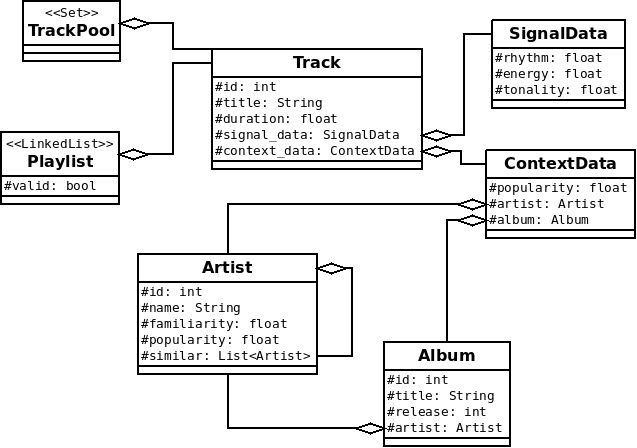
\includegraphics[width=\textwidth]{data/archi/track.png}
\caption{Diagramme des classes constituant un morceau.}
\end{figure}

Il a été décidé de séparer les informations du morceaux selon deux thèmes bien
distincts~:
\begin{description}
  \item[Liées au signal~:] Les données liées au signal sont directement reliées
  aux données du signal musical (ex. tempo).
  \item[Liées au conntexte~:] Les données liées au contexte n'ont pas de 
  lien avec le signal, mais décrivent plutôt l'environnement du morceau 
  (ex. popularité, artiste, etc.).
\end{description}

Toutes les classes et sous-classes d'un morceau utilisent des accesseurs car 
leurs attributs ne doivent pas être modifiés après la sélection.

Deux structures de données sont utilisées pour contenir des ensembles de
morceaux~:
\begin{description}
  \item[Playlist~:] Une liste chainée, ce qui permet d'ajouter des éléments en
  complexité constante. De plus elle comporte un attribut qui atteste de sa validité.

  \item[TrackPool~:] C'est la structure qui est renvoyée par le module de 
  données (interface IDatabase cf. \ref{archi:generation:database}). La
  complexité est bonne pour la recherche, l’itération, et l'insertion. De plus,
  les éléments insérés ne peuvent pas être modifiés.
\end{description}

\subsubsection{Données Signal}

\begin{description}
  \item[Rythme~:] Descripteur définissant si le morceau est rythmé. Il
  représente un score entre 0 et 1, exprimable en pourcentage.
  \item[Énergie~:] Décrit la puissance du morceau, la densité de son. C'est
  aussi un score entre 0 et 1, tout comme le rythme.
  \item[Tonalité~:] Représente la note et le mode (ex majeur ou mineur) du 
  morceau\footnote{Ce descripteur n'a pas pu être implémenté, d'une part à
  cause de la difficulté à trouver une structure pour le contenir, et d'autre
  part à cause de la faible fiabilité des valeurs liées dans la MSD}.
\end{description}

\subsubsection{Données de Contexte}

\begin{description}
  \item[Popularité du morceau~:] Un score décrivant la popularité de morceau,
  varie en fonction du temps.
  \footnote{N'est pas très utilisé, car souvent non rempli dans la MSD. De
  plus, comme nous utilisons une base de données statique, et que cette valeur
  tends à changer, elle se retrouve finalement assez obsolète}

  \item[Artiste~:] Représente l'artiste/groupe auteur du morceau.
  % TODO

  \item[Album~:] Représente l'album dont est issu le morceau.
  %TODO

  Il est important de noter que contrairement au diagramme UML, la liste
  d'artistes similaires contient uniquement les identifiants des artistes 
  afin d'éviter des inclusions cycliques.
\end{description}

\subsection{Options:~ La classe OptionList}
\label{archi:communication:options}

Il était important d'utiliser un objet pour passer les options entrées par
l'utilisateur. Ceci permet d’éviter de donner trop de paramètres aux fonctions
du module de génération. De plus, cette structure peut être modifiée pour
permette de passer de nouvelles options.

Pour éviter les erreurs, cette classe ne peut pas être modifiée après son
instanciation.

\section{Génération}
\label{archi:generation}

\begin{figure}[H]
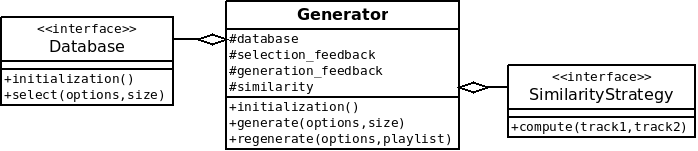
\includegraphics[width=\textwidth]{data/archi/generator.png}
\caption{Diagramme des classes du générateur.}
\end{figure}

Le module de génération s'occupe de la création de la playlist. 
L'interface utilisateur appelle toutes les fonctions du module 
de génération, et celui-ci appelle à son tour toutes les fonctions des deux 
autres sous-modules. La fonction \texttt{initialization} sert à vérifier la 
présence d'une base de données lors du démarrage du programme. 

\subsection{Le cœur de la génération~: La classe Generator}
\label{archi:generation:generator}

La classe Generator est en lien direct avec l’interface. Elle a le rôle de chef
d'orchestre, car elle va utiliser les sous-modules qui lui sont liés pour
construire une playlist.

\subsection{Interface avec les données~: L'interface IDatabase}
\label{archi:generation:database}

Le module de données (SQLiteDatabase) a pour objectif d'assurer la 
communication entre le module de génération et la base de données utilisée. 
Sa principale fonctionnalité est d'effectuer une sélection dans la base de 
données en fonction du nombre de chansons souhaité et des paramètres de 
sélection entrés par l'utilisateur. Cette opération se fait grâce à la 
fonction \texttt{select}. De plus, lors du lancement du programme, une 
fonction d'initialisation est appelée afin de certifier la présence de la 
base de données.
Cette interface permet au générateur d'aller chercher des données dans le
conteneur de notre choix (une base de données SQLite dans notre cas), juste
en créant une classe implémentant cette interface.

\subsection{Stratégie de similarité~: l'interface ISimlarityStrategy}
\label{archi:generation:similarity}

Cette interface utilise le design pattern \emph{Strategy} pour permettre de
changer le comportement de la similarité dans le générateur. Pour cela,
la méthode \texttt{compute} est virtuelle. Grâce à cela, si une implémentation
de cette interface est réalisée (dans notre cas la classe SimilarityStrategy),
on peut passer par une référence de ISimilarityStrategy pour appeler notre
implémentation. Les comportements sont donc potentiellement illimités, et ce
en changeant uniquement l'attribut \texttt{similarity} du générateur.

\section{Module de sortie}
\label{archi:sortie}

Le module de sortie (ici TextOutput) est en charge de fournir à 
l'utilisateur un moyen de récupérer le résultat de la génération demandée. 
Ce module (ainsi que tous les modules de sortie pouvant être crées) devront 
respecter l'interface OutputStrategy pour pouvoir être utilisés sur le 
programme. Dans le cas du module TextOutput, le résultat obtenu sera mis 
sous la forme d'un fichier texte contenant les titres, artiste, album et années 
des différents morceaux de la playlist. Cette fonctionnalité est assurée par la fonction 
\texttt{format} à laquelle on passe la playlist générée en paramètre.

Nous disposons d'un deuxième module de sortie (TextIDOutput), fonctionnant comme
le précédent, mais ne place que les ID (ici Echo Nest dans notre base de données)
des morceaux dans le fichier.

\section{Interface Utilisateur}
\label{archi:interface}

L'Interface Utilisateur (UserInterface) se charge de faire le lien entre
l'utilisateur et le programme. Sa fonction principale est de lancer une
génération de playlist en appelant la fonction \texttt{generate} du module de 
génération. Lors de l'appel à cette fonction, les informations rentrées par 
l'utilisateur sont transmises en paramètres. Lors du lancement du programme,
une fonction d'initialisation est lancée. Cette dernière permet d'assurer 
la présence de la base de données ainsi que du, ou des, module(s) de sortie.

\subsection{Interface Utilisateur Console}
\label{archi:interface:console}

L'interface utilisateur console (ConsoleUserInterface) dispose de toutes les options 
nécéssaires au lancement d'une génération. 
Elle doit être executée via la commande suivante :

\texttt{./soundcitybash <database>}

(\texttt{<database>} désignant l'emplacement vers la base de données).

\vspace{3mm}
\noindent L'utilisateur peut lancer le programme en utilisant les options suivantes :
\begin{itemize}
\item \texttt{-h} : Affiche l'aide
\item \texttt{-y <startYear[1-3000]> <endYear[1-3000]>} : Définit un intervalle 
d'années pour les morceaux.
\item \texttt{-e <energy[0.0-1.0]>} : Impose une valeur d'énergie dans 
la playlist générée.
\item \texttt{-p <popularity[0.0-1.0]>} : Impose une valeur de popularité 
dans la playlist générée.
\item \texttt{-r <rhythm[0.0-1.0]>} : Impose un rythme dans la 
playlist générée.
\item \texttt{-m <mood[0.0-1.0]>} : Impose une humeur dans la 
playlist générée (plus la valeur est élevée, plus le morceau est joyeux).
\item \texttt{-s <size[1-100]>} : Choix de la taille de la 
playlist générée (10 par défaut).
\item \texttt{-o <fileName>} : Choix du nom du fichier de sortie.
\item \texttt{-a < "Artist Name" >} : Impose un artiste.
\item \texttt{-id} : Le fichier de sortie ne contiendra que les ID Echo Nest 
des morceaux de la playlist
\item \texttt{-v} : Active le mode verbeux (feedback).
\end{itemize}

\subsection{Retour utilisateur}
\label{archi:interface:feedback}

Le retour utilisateur permet de notifier l'interface de l’avancement de la génération, 
de façon simple, en utilisant les design patterns \emph{Observable}
et \emph{Observer}.

\begin{figure}[H]
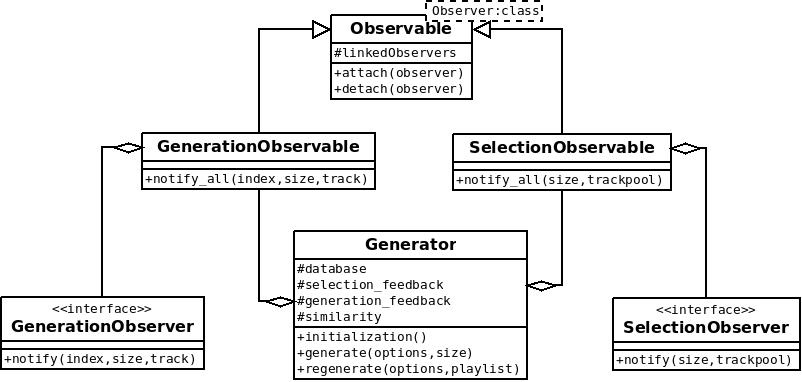
\includegraphics[width=\textwidth]{data/archi/feedback.png}
\caption{Diagramme des classes servant au retour utilisateur.}
\end{figure}

Pour ajouter un retour utilisateur, il faut donc implémenter un Observer, en
fonction de la phase dont on veut avoir le retour. Cette implémentation passe
surtout par la méthode \texttt{notify}, qui sera appelée par l'Observer.
Ensuite, il suffit d'attacher notre Observer à l'Observable lié dans le
générateur (grâce à la méthode \texttt{attach}).

La classe parente des Observable, qui est aussi la seule classe template du
projet, permet d'éviter la duplication de code. En effet, les classes dérivant
d'Observable ont un comportement similaire, sauf au niveau de leur méthode
\texttt{notifyAll}.

\begin{figure}[H]
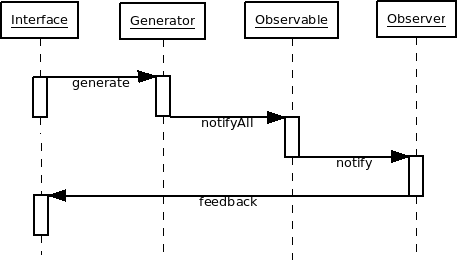
\includegraphics[width=\textwidth]{data/archi/feedback_sequence.png}
\caption{Diagramme de séquence du retour utilisateur.}
\end{figure}

L'utilisation des designs patterns est ici assez simple. Les deux types
d'Observable sont contenus dans le générateur, qui appelle leur méthode
\texttt{notifyAll} au moment opportun. Ainsi, la méthode \texttt{notify} des 
Observers liés est appelée, produisant le retour utilisateur qu'ils ont
implémentés.
